\section{Strategy}
\label{Strategy}
We find it interesting to research the design of smarter players, who take into account board characteristics when deciding which marble to place or which sub-board to rotate.
There are two players in the game. Each player has a flag if he is employing a specific strategy or plays randomly. 
To compare two players we use a monte carlo style method: We execute a number of playthroughs until one of the final states is achieved(draw or a player wins).
From these playthroughs we gather the execution time, the number of transitions taken and the result of the game.

\vspace{6pt}
\subsection{Algorithm}
The developed strategy is to extend a row of marbles until five in a row has been achieved(and the game is won).
If there is an existing row it will try to extend the longest row.
If there isn't a row,or if there are no rows that can be extended a new row will be started.
 In order to achieve this it has two main rules:
\begin{itemize}
\item Try to extend the longest consecutive row of marbles of its color.
\item Place a marble in a center position
\end{itemize}
Both rules will be discussed in the rules paragraph.
In order to make decisions it first tries to look for a row of 4 marbles and places one marble at either possible end. If this is not available it looks for a row of 3. This patern repeats till the length of the row is 1.
If it can not find a free Space adjacent to a marble of its own, then it will try to occupy a Space in the center of a block.
If none of the strategy rules can be matched, the system will fall back by placing a marble in a random empty Space.
This algorithm has been implemented in the control program.
Rules and control programs to model the strategy are placed in the "strategy" folder/ package.

\subsubsection{Control Program}

The algorithm  has its own control program in the strategy package to enforce the order in which the rules are matched.
\lstset{ %
	language=C++,                % choose the language of the code
	basicstyle=\footnotesize,       % the size of the fonts that are used for the code
	numbers=left,                   % where to put the line-numbers
	numberstyle=\footnotesize,      % the size of the fonts that are used for the line-numbers
	stepnumber=1,                   % the step between two line-numbers. If it is 1 each line will be numbered
	numbersep=5pt,                  % how far the line-numbers are from the code
	backgroundcolor=\color{white},  % choose the background color. You must add \usepackage{color}
	showspaces=false,               % show spaces adding particular underscores
	showstringspaces=false,         % underline spaces within strings
	showtabs=false,                 % show tabs within strings adding particular underscores
	frame=single,           % adds a frame around the code
	tabsize=2,          % sets default tabsize to 2 spaces
	captionpos=b,           % sets the caption-position to bottom
	breaklines=true,        % sets automatic line breaking
	breakatwhitespace=false,    % sets if automatic breaks should only happen at whitespace
	escapeinside={\%*}{*)}          % if you want to add a comment within your code
}

\begin{lstlisting}
function pm() {
try {
	add2fourLeft|add2fourRight;
}else{
	try{
		add2threeRight|add2threeLeft;
	}else{
		try{
			add2twoLeft|add2twoRight;
		}else{
			try{
			add2oneLeft|add2oneRight;
		}else{
			try{
				midBlock;
			}
			else{
				placeMarble;
			}
		}
	}
}
}
}
\end{lstlisting}
The function "pm" (short for place marble) first tries to match one of the rules to extend 4-in-a-row, then for 3 and so on. If no row can be extended the "midBlock" rule  places a marble in the center of a block. If none of these rules can be matched a random marble is placed somewhere on a free spot.

To make sure that a player uses its appointed strategy, the "game\_progress" control program in the main package was also updated.
The "executePlace" function first tries to match strategy rules by calling the "pm" function of the strategy. If none of these rules match, either because the player has no strategy flag or because the strategy is exhausted, then it will try to match the general "placeMarble" rule. 
In our case this is ultimately not necessary but it ensures that the game will always progress in case of a faulty algorithm

\subsubsection{The graph production systems}
This section describes the special graph production systems(also called rules) for executing the strategy.

\begin{figure}[!h]
  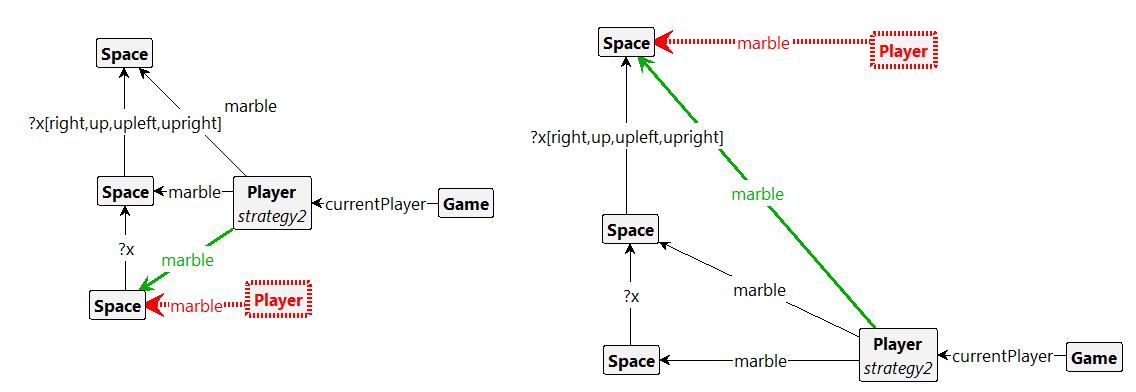
\includegraphics[scale=0.5,clip]{Images/twocombined.png}
  \caption{Two ways of extending a row}
  \label{fig:twocombined}
\end{figure}

The most interesting rule is the extending of an existing row. Edges are one directional, because of this we get two rules for this situation: one for placing a marble at the "beginning" end of the row and one to add to the "end" of the row. Depicted is the rule for extending a row of length 2. Similar rules have been made for rows of length four, two and one.\\
These rows' can be in 4 different directions. To prevent a blowup in the number of rules we chose to use a wildcart for the direction edges, that have to match with "up", "down", "downleft" or "downright".
This does make the matching somewhat slower, since these rules are harder to match. However we feel it is justified because otherwise we would need 4 times the 4 rules to model each direction.

If there is no existing row to extend, the algorithm tries to place a marble in the center space of a block. This can easily be done by matching on the "place5" flag that is already present on the board. This is done in the "midBlock" rule.

The algorithm has no strategy for turning blocks, there are no additional rules or control programs needed for this part of the game.


\subsection{Results}
To be able to draw a conclusion about whether our strategy performs well, we want to formally evaluate its performance.
Because the game is relatively complex, it is impossible to generate the entire state space of the game, and determine the complete win rate of the naive and the smart strategies.
Therefore we have decided to perform a Monte Carlo simulation. A Monte Carlo simulation produces distributions of possible outcome values.

\vspace{6pt}

TODO

To determine the number of iterations needed to meet these requirements, we use the following formula \cite{sim-modeling}:

%n = (zα/2 S / E ) ²
